\setchapterimage[7.5cm]{images/jong-marshes-79mNMAvSORg-unsplash}
\setchapterpreamble[u]{\margintoc}
\chapter{Control Flow Testing}
\section{Introduction}
Control flow testing is a software testing  strategy that depicts the execution order of the assignment and control statements in a program unit such as a function. This strategy is implemented by developing test cases of a unit and executing and tracing the execution flow. Flow of execution of the assignment and I/O statements in a program unit is sequential and change whenever a control statement (if-then-else, for, switch/case and while) is encountered and executed. A program unit has an entry and an exit point. Commands in a program unit are executed from the command at the entry point to the command at the exit point, depending on the program flow. The sequence of these flow steps is defined as the program execution path. Depending on the number and complexity of control commands, multiple paths can occur in a unit. The paths in the program are shaped depending on the input values in the program unit.

A program unit can have multiple paths. Testing all paths with the input value that determines the path is not a very efficient approach and is costly. There are many approaches to increasing testing efficiency and minimizing its cost. The McCabe cyclomatic complexity analysis is one of them and will be discussed in the following sections.

The control flow testing steps are summarized below:
\begin{enumerate}
    \item Creation of control flow graph (CFG).
    \item Determination of the path to be tested according to the path selection criteria.
    \item Creation of necessary inputs and relevant test case for the determined path.
\end{enumerate}
Path selection criteria will be discussed in detail in the next subsections.

\section{Control Flow Graph (CFG)}
A control flow graph\index{control flow graph (CFG)} is a directed graph with an entry and an exit point. It is similar to a flowchart and is used to represent the overall flow in a unit. In a CFG, a rectangular node represents a sequential computation encompassing a set of statements in order, a decision node is used for branching (if-then-else), and a circle represents a merge point. A directed edge is used to connect nodes. In order to identify a path uniquely, each node is labeled with a unique integer. A decision node provides branching to the sides of the box by a True (T) or a Yes (Y) label. A complete execution path in a CFG is defined with a set of ordered nodes from 1 to N, where 1 and N are the labels of the entry point, and the exit point respectively. The basic nodes of a CFG is shown in \reffig{fig:cfg-31}.

\begin{figure}[!ht]
    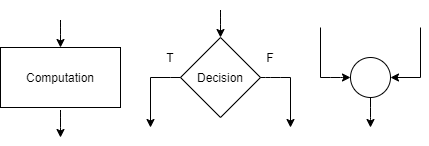
\includegraphics{images/cfg-figure-3-1.png}
    \caption{Basic nodes (computation, decision and merge) in a CFG.}
    \labfig{fig:cfg-31}
\end{figure}

Using these nodes one can construct CFG elements for the basic programming structures (selection/if-then-else, multi-way branching/switch or case, and iteration/while-do or repeat-until). Some of these CFG constructs are shown in \reffig{fig:cfg-32}.

\begin{figure}[!ht]
    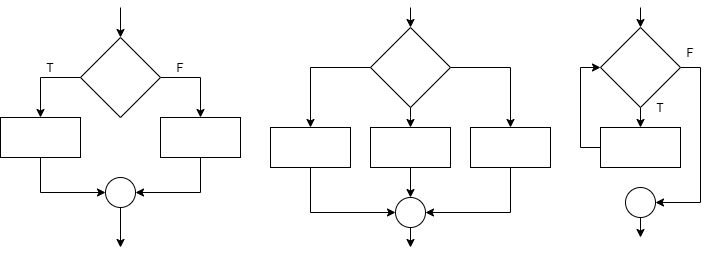
\includegraphics{images/cfg-figure-3-2.png}
    \caption{if-then-else, switch, and while-do constructs in a CFG.}
    \labfig{fig:cfg-32}
\end{figure}

Other constructs such as repeat-until, nested if, and for loop structures can be constructed in a similar way from these basic constructs.

\begin{exercise}
\labexercise{cfg-exercise}
For the C program below, create a CFG and identify the paths.
\begin{lstlisting}[language=C, caption={A C program that prints the negative integers in an array of 10 integer values.}]
#include <stdio.h>
int main(){
  int array[10] = {-11, 24, 32, -7, 28, 14, 1, -3, -16, 21};
  int k = 0, count = 0;
  printf("Displaying negative integers:\n");
  while (k <= 10){
  	if (array[k] < 0){
  		printf("%d\n", array[k]);
		count++;  	
    }	 
	k++;
  }
  printf("Number of negative integers:%d\n", count);
  return 0;
}
\end{lstlisting}
\end{exercise}

\begin{marginfigure}
    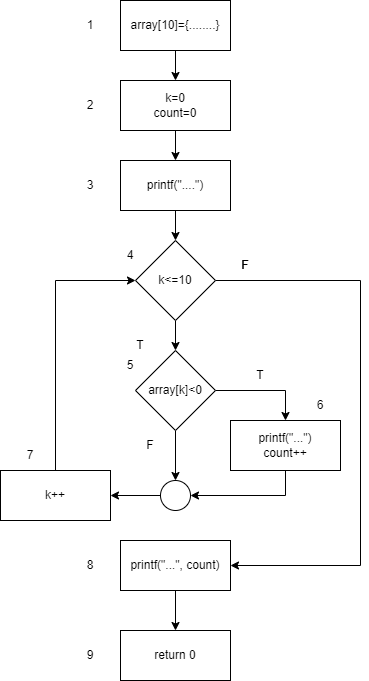
\includegraphics{images/cfg-figure-3-3.png}
    \caption{A CFG for the C program given in \refexercise{cfg-exercise}.}
    \labfig{fig:cfg-33}
\end{marginfigure}

A CFG for this program is given in \reffig{fig:cfg-33}.

Some of the paths are identified as follows:
\begin{itemize}
    \item Path1: 1-2-3-4(F)-8-9
    \item Path2: 1-2-3-4(T)-5(T)-6-7-4(F)-8-9
    \item Path3: 1-2-3-4(T)-5(F)-7-4(F)-8-9
    \item Path4: 1-2-3-4(T)-5(T)-6-7-4(T)-5(F)-7-4(F)-8-9
\end{itemize}

\section{McCabe Cyclomatic Complexity}
The concept of cyclomatic complexity metric of a software unit is first defined by McCabe in 1976 \autocite{mccabe1976complexity}. Given a program unit, and a corresponding flow graph (program graph) G with N nodes and E edges, the cyclomatic complexity of the graph $V(G)$ is computed using the formula $V(G) = E - N + 2$. V(G) is always greater than or equal to 1. Each node in the graph $G$ indicates one or more statements (assignment, I/O or control) in the program and the flow of control is represented by directed edges. The basic structures in the McCabe complexity graph are the same as those in the CFG. However, in the McCabe graph, the decision nodes and assignment statement nodes are represented as circled nodes. The CFG given in \reffig{fig:cfg-33} is redrawn in \reffig{fig:cfg-34} using the McCabe graph notation. For simplicity, some of the nodes representing the initialization (assignment) statements are merged into a single node.

\begin{marginfigure}[-4cm]
    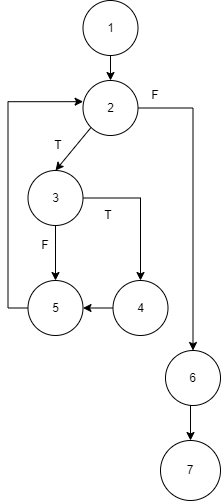
\includegraphics{images/cfg-34.png}
    \caption{McCabe program graph for the C program given in \refexercise{cfg-exercise}.}
    \labfig{fig:cfg-34}
\end{marginfigure}

Cyclomatic complexity of this graph is simply $V(G) = E - N + 2 = 8 - 7 + 2 = 3$. Three independent paths are shown below:
\begin{itemize}
    \item Path1: 1-2(F)-6-7
    \item Path2: 1-2(T)-3(T)-4-5-2(F)-6-7
    \item Path3: 1-2(T)-3(F)-5-2(F)-6-7
\end{itemize}

The McCabe complexity metric guides the tester about the number of paths to be tested by providing the number of independent paths in the program graph. Independent path is defined as a path that has at least one edge which has not been traversed before in any other paths. In the  software world, it is generally accepted or tried case that this complexity value is less than ten. It is common practice to simplify or subdivide a unit into manageable units with values greater than ten.

\section{Path Selection Criteria}

\subsection{All-paths Coverage}

\subsection{Statement Coverage}

\subsection{Branch Coverage}

\subsection{Predicate Coverage}

\section{Generating Test Cases}

\section{Problems}
\begin{enumerate}
    \item Create a CFG for the \lstinline!BinarySearch! function given in \refexercise{ex22}. Give a list of possible paths.
    \item Write a C function to sort n integers in descending order using Bubble sort. Draw the McCabe program graph and compute the McCabe cyclomatic complexity for this program and state the number of independent paths accordingly.
    \item Write a C function to find the greatest common divisor (GCD) of two integers M, and N by using the Euclidean algortihm.Draw the McCabe program graph, compute the McCabe cyclomatic complexity for this program and state the number of independent paths accordingly.
    The pseudo-code of the Euclidean algorithm is given below:
    \begin{itemize}
        \item Step 1: Let  a, b  be the two non-negative integers
        \item Step 2: Let R = a mod b 
        \item Step 3: Let  a = b  and  b = R
        \item Step 4: Repeat Steps 2 and 3 until  a mod b  is greater than 0
        \item Step 5: GCD = b
        \item Step 6: End
 \end{itemize}
    \item 
    \item 
    \item
    \item 
\end{enumerate}